%!TEX root = ../bachelor.tex
\chapter{Fazit und Ausblick}
Parallelisierung?
geht immer, weil Imageprocessing.

hough evtl besser probalistic oder richtungasinformationen mit nehmen

splatting

iteratives verfahren zum minimieren des reprojection fehlers ausprobieren
robustes projektionsgedöns

Um die Löcher bei der Vörwärtsentfalung zu schließen, könnte man eine Delaunay-Triangulation durchführen. 
Da das Verfahren jedoch ohne Triangulation schon relativ rechenintensiv ist, und die Rückwärtsentfaltung sehr gute Ergebnisse liefert wurde dieses Möglichkeit nicht weiter untersucht.
\begin{figure}[!htb]
	\centering
	\begin{subfigure}{.9\textwidth}
		\centering
		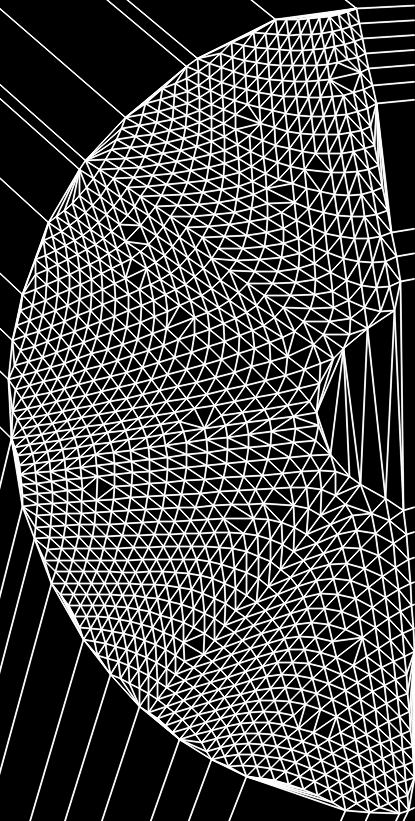
\includegraphics[angle=-90, width=.8\textwidth]{images/delaunay1.png}
		\caption{Triangulation mit $10\%$ der Punkte}
	\end{subfigure}
	\begin{subfigure}{.9\textwidth}
		\centering
		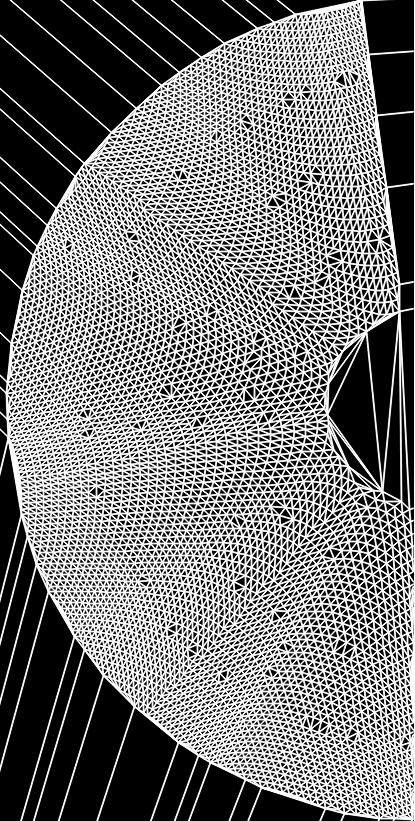
\includegraphics[angle=-90, width=.8\textwidth]{images/delaunay2.png}
		\caption{Triangulation mit $40\%$ der Punkte}
	\end{subfigure}
	\label{fig:delaunay}
	\caption{Delaunay-Triangulation}
\end{figure}

\begin{equation}
	G(x,y) = \frac{((x - x_0)\cos\theta + (y - y_0)\sin\theta)^2}{a^2} + \frac{((x - x_0)\sin\theta - (y - y_0)\cos\theta)^2}{b^2} - 1 = 0
\end{equation}

\begin{equation}
	E = E_M + E_A + E_S
\end{equation}

\begin{equation}
\begin{aligned}
E_M &= -\alpha\frac{1}{n}\sum_{i=0}^{n-1}I_M(p_i) \\
E_A &= \beta\frac{1}{n}\sum_{i=0}^{n-1}\left(I_O(pi) - \atant{\left(\frac{\partial G}{\partial y}(p_i), \frac{\partial G}{\partial x}(p_i)\right)}\right)^2 \\
E_S &= \gamma\frac{1}{n}\sum_{i=0}^{n-2}\abs{p_i - p_{i+1}}
\end{aligned}
\end{equation}

Man macht die Initialellipse möglichst größ und bestimmt dann numerisch, beispielsweise durch Gradient Descent, ein Minimum der Funktion. Der Term $E_M$ wird minimal, wenn entlang der Ellipse die Kantenstärke (\textit{\textbf{M}agnitude}) groß ist. Der Term $E_A$ wird minimal wenn die Winkel der Normalenvektoren ähnlich zu denen der Kanten sind (\textit{\textbf{A}ngle}) und $E_S$ wird minimal, wenn die Distanz aufeinanderfolgender Ellipsepunkte klein wird, also die Ellipse als ganzes klein wird (\textit{\textbf{S}ize}). Der Term lässt die Ellipse also schrumpfen. $\alpha, \beta$ und $\gamma$ steuern hierbei den Einluss der einzelnen Terme. Das Problem bei diesem Ansatz, ist dass die Funktion auch nach starker Gaussglättung, schnell in kleine lokale Minima läuft, obwohl ein wesentlicher stärkeres Minimum in näherer Umgebung wäre. Darüber hinaus muss für ein robustes Optimierungsverfahren der Gradient und im Besten Fall sogar die Hesse-Matrix zur Verfügung gestellt werden. 



\todo{Literatur checken, ins besondere seitenangaben}